\documentclass[12pt, a4paper]{scrartcl}
\usepackage[left=4cm,right=2cm, top=3cm, bottom=3cm]{geometry}
\usepackage[T1]{fontenc}
\usepackage[utf8]{inputenc}
\usepackage[ngerman]{babel}
\usepackage{lmodern}
\KOMAoption{listof}{entryprefix}


% =================== - TEXT - =========================
% for header in komascript documents
\usepackage[automark,headsepline]{scrlayer-scrpage}
\clearpairofpagestyles
\pagestyle{scrheadings}
\setkomafont{pageheadfoot}{}
\ihead{\leftmark}
\cfoot*{\pagemark} %Pages for heading and plain pages
\usepackage{enumitem}
\usepackage{hyperref}

% heading spacing
\usepackage[onehalfspacing]{setspace}
\parindent 0pt
\parskip 1.5em
% text symbols
\usepackage{textcomp}
\usepackage{tabto}

% =================== - Tables - =====================
\usepackage{tabularx}
\usepackage[table]{xcolor}

% =================== - GRAPHICS - =====================
\usepackage{float}
\usepackage{graphicx}
\usepackage{caption}
\usepackage{subcaption}


% =============== - MUSIC - =========================
\usepackage[chorded]{songs} % Paket fuer Akkorddiagramme
\usepackage{harmony}



\newcommand{\RomanNumeralCaps}[1]
    {\MakeUppercase{\romannumeral #1}}

% ======================================================
%					- END OF PREAMBLE -
% ======================================================

\begin{document}

% ========= - TITLE AND NONPAGECOUNT SITES - ============
\pagenumbering{Roman}
\begin{titlepage}

    \vspace{20mm}

    \centering
    \huge\textbf{Blues}\par
    \vspace{3mm}

    \begin{figure}[htbp]
        \centering
        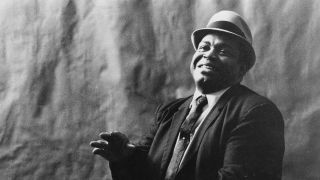
\includegraphics[width=0.8\textwidth]{images/title_img}
    \end{figure}

    \vspace{3mm}
    \textsc{\LARGE{Mathias Gewissen}}\par
    \vspace{3mm}
    \large Untertitel \par

\end{titlepage}
\thispagestyle{plain}
\tableofcontents

% ================= - MAIN TEXT PART - =================

\newpage
\pagenumbering{arabic}
\section{Einleitung}
Die Musiktheorie gliedert sich in Harmonie- und Tonsatzlehre, Analyse, 
Formenlehre, Gehörbildung, Höranalyse, Improvisation und Komposition.
Musiktheorie erklärt, wie Musik funktioniert. Sie ist die Struktur, die einem Song zugrunde liegt und erklärt, wie sie funktionieren. Doch Musiktheorie kann 
auch den Weg nach vorne weisen. Zumindest die Grundlagen der Theorie zu lernen ist ein 
unumgänglicher Teil der musikalischen Entwicklung. Am Anfang kann die Theorie etwas 
einschüchternd wirken. Das Thema ist so groß, dass es schwer ist zu wissen, wo man am 
besten anfängt. Dies ist ein Leitfaden, der dabei hilft, mit der Musiktheorie 
loszulegen, sodass die Grundlagen leicht verstanden werden und sie korrekt auf eigene 
Musik angewendet werden können.

\newpage
\section{Grundlagen}
\subsection{Ton und Tonstufe}
    \textbf{Die Tonstufe} ist ein einzelner Ton einer diatonischen Tonleiter. Als Kernbestand des abendländischen Tonsystems kann man die sieben Tonstufen \textbf{C, D, E, F, G, A und B ansehen, die Stammtöne.} Zwichen den Tonstufen liegt jeweils immer ein Halbtonschritt. Die Tonstufen einer gegebenen Tonleiter werden mit lateinischen Ordinalzahlen benannt.

\begin{table}[H]
    \caption{Tonstufen Steigend}
    \label{tab:TonstufenSteigend}
    \begin{tabularx}{\textwidth}{|>{\hsize=.3\hsize}X|>{\hsize=.3\hsize}X|>{\hsize=.4\hsize}X|}
    \hline
    Halbtönschritte & Ton & lateinische Ordinalzahlen\\ \hline
    0 & \textbf{C} & \textbf{Reine Prime} \\ \hline
    1 & Cis & Kleine Sekunde \\ \hline
    2 & \textbf{D} & \textbf{Große Sekunde} \\ \hline
    3 & Dis & Kleine Terz \\ \hline
    4 & \textbf{E} & \textbf{Große Terz} \\ \hline
    5 & \textbf{F} & \textbf{Quarte} \\ \hline
    6 & Fis & Tritonus \\ \hline
    7 & \textbf{G} & \textbf{Reine Quinte} \\ \hline
    8 & Ais & Kleine Sexte \\ \hline
    9 & \textbf{A} & \textbf{Große Sexte} \\ \hline
    10 & Bb & Kleine Septime \\ \hline
    11 & \textbf{B} & \textbf{Große Septime} \\ \hline
    12 & \textbf{C} & \textbf{Reine Oktave}\\ \hline
    \end{tabularx}
\end{table}

Grundsätzlich betrachten wir die Tonleitern in steigender oder fallender Reihenfolge. Wir erkennen, dass bestimmte Töne zwar verschieden geschrieben werden, jedoch gleich klingen. Ein \textbf{Cis} bspw. klingt wie ein \textbf{Des}. Sie dir dazu mal den Halbtonschritt 1 in der Tabelle \ref{tab:TonstufenSteigend} an und in der Tabelle \ref{tab:TonstufenFallend} den Halbtonschritt 11. Hauptsächlich hat das etwas mit dem Vorzeichen (Versetzungszeichen) zu tun. Das hier erstmal nicht weiter beachtet werden soll.

\begin{table}[H]
    \caption{Tonstufen Fallend}
    \label{tab:TonstufenFallend}
    \begin{tabularx}{\textwidth}{|>{\hsize=.3\hsize}X|>{\hsize=.3\hsize}X|>{\hsize=.4\hsize}X|}
    \hline
    Halbtönschritte & Ton & lateinische Ordinalzahlen\\ \hline
    0 & \textbf{C} & \textbf{Reine Prime} \\ \hline
    1 & B & Kleine Sekunde \\ \hline
    2 & \textbf{Bb} & \textbf{Große Sekunde} \\ \hline
    3 & A & Kleine Terz \\ \hline
    4 & \textbf{As} & \textbf{Große Terz} \\ \hline
    5 & \textbf{G} & \textbf{Quarte} \\ \hline
    6 & Ges & Tritonus \\ \hline
    7 & \textbf{F} & \textbf{Reine Quinte} \\ \hline
    8 & E & Kleine Sexte \\ \hline
    9 & \textbf{Es} & \textbf{Große Sexte} \\ \hline
    10 & D & Kleine Septime \\ \hline
    11 & \textbf{Des} & \textbf{Große Septime} \\ \hline
    12 & \textbf{C} & \textbf{Reine Oktave}\\ \hline
    \end{tabularx}
\end{table}

Wir fassen alle einzelnen Töne noch einmal zusammen. Töne die gleich klingen aber 2 Bezeichnungen haben, werden im Übrigen enharmonische Töne genannt. In der oberen Zeile in Tabelle \ref{tab:ToeneUndHalbtoene} lesen wir die Töne steigend (C, D, E, usw.) und hängen ein -is- an. Wird wie in der unteren Zeile fallend gelesen (C, B, Bb, A, usw.), wird ein -es- angehangen. Aus A wird jedoch As und aus B wird Bb.

\begin{table}[H]
    \caption{Töne und Halbtöne}
    \label{tab:ToeneUndHalbtoene}
    % \begin{tabularx}{\textwidth}{|*{12}{X|}}
    \begin{tabularx}{\textwidth}{|p{1.2cm}|p{1.2cm}|X|X|X|p{1.2cm}|X|X|X|X|X|X|}
    \hline
    \cellcolor{red!25}His/C & \cellcolor{yellow!25}Cis & D & \cellcolor{green!25}Dis & E & \cellcolor{red!25}Eis/F & \cellcolor{gray!25}Fis & G & \cellcolor{blue!25}Gis & A & \cellcolor{orange!25}Ais & B \\ \hline
    C & \cellcolor{red!25}Ces/B & \cellcolor{orange!25}Bb & A & \cellcolor{blue!25}As & G & \cellcolor{gray!25}Ges & F & E & \cellcolor{green!25}Es & D & \cellcolor{yellow!25}Des \\ \hline
    \end{tabularx}
\end{table}

Lass dich von den rot markierten Zellen nicht verwirren. Sie stehen für sich. Lesen wir steigend (also die obere Zeile) und sind beim B angekommen geht es von vorn los und somit ist C auch gleichzeitig ein His. Genauso ist es wenn wir fallend lesen. Hier ist der Ton B und Ces der gleichklingende. Auch zwischen E und F liegt nur ein Halbtonschritt, sodass Eis und F derselbe Ton ist.

\subsection{Tonarten}
Tonarten sind Sequenzen aus natürlichen Tönen mit Vorzeichen. Es gibt zwei Vorzeichen. Das \textbf{Kreuz \# und Das b.} \textbf{Die Anzahl der Töne innerhalb einer Tonleiter die ein -is- bekommen und erhöt werden müssen, entspricht immer der Anzahl der Kreuze \#.} \textbf{Die Anzahl der Töne innerhalb einer Tonleiter die ein -es- bekommen und erniedrigt werden müssen, entspricht immer der Anzahl der b's.} Die Tonart C-Dur besteht komplett aus natürlichen Tönen ohne Vorzeichen: C – D – E – F – G – A – B. Die Tonart G-Dur besteht aus einem Vorzeichen G – A – B – C – D – E – F\#. Im Gegensatz dazu beinhaltet die Tonart \textbf{Cis-Dur} ausschließlich Töne mit Kreuzen: \textbf{C\# – D\# – E\# – F\# – G\# – A\# – B\#.} Erkennen kannst du es immer an den Vorzeichnen die vor dem Notenschlüssel stehen.

\begin{minipage}[b]{0.3\linewidth}
    \begin{figure}[H]
        \centering
        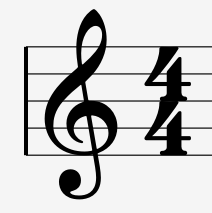
\includegraphics[width=0.4\textwidth]{images/Signiture_2}
        \caption[]{C-Dur}
        \label{fig:CDur}
    \end{figure}
  \end{minipage}
  \begin{minipage}[b]{0.3\linewidth}
    \begin{figure}[H]
        \centering
        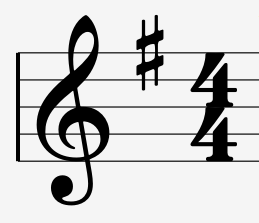
\includegraphics[width=0.45\textwidth]{images/Signiture_3}
        \caption[]{G-Dur}
        \label{fig:GDur}
    \end{figure}
  \end{minipage}
  \begin{minipage}[b]{0.3\linewidth}
    \begin{figure}[H]
        \centering
        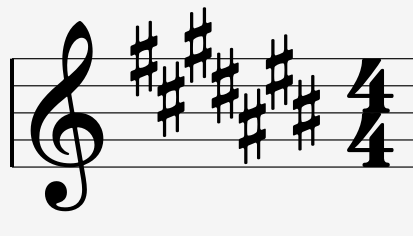
\includegraphics[width=0.65\textwidth]{images/Signiture_1}
        \caption[]{Cis-Dur}
        \label{fig:CisDur}
    \end{figure}
  \end{minipage}

\subsection{Tonleitern}
Eine Tonleiter oder Ton-Skala ist in der Musik eine Reihe von der Tonhöhe nach geordneten Tönen. In den meisten Fällen hat eine Tonleiter den Umfang einer Oktave. Weit verbreitet sind diatonische Tonleitern in Dur und Moll. Tonleitern sind durch Tonabstände definiert. An erster Stelle steht der Grundton (wie zum Beispiel C) nach 8 Tönen (also einer Oktave) wiederholt sich die Reihe. Der 8. Ton ist also wieder ein C. 
\textbf{Die Verbindung des Tongeschlechts, also bspw. Dur oder Moll, mit dem Grundton ergibt die Tonart}. 
C-Dur ist hierfür ein Beispiel. Weitere sind A-Moll, D-Dur usw.

Eine Dur-Tonleiter wird ausgehend vom Grundton gebildet, indem jeweils ein Ganztonschritt weiter 
gesprungen wird. Die \textbf{Stellen von Ton 3 zu 4 und von Ton 7 zu 8. sind Ausnahmen. Hier wird nur ein
Halbtonschritt gesprungen.} Analog wird diese Verfahrensweise auch für alle weiteren Grundtöne angewendet. 
In der Tabelle sind die gebräuchlichsten Dur Tonleitern angegeben. Die Farben markieren den Halbtonschritt. Schau dir genau an welche Töne ein -is- bekommen.

\begin{table}[H]
    \caption{Gebräuchlichste Dur-Tonleitern}
    \label{tab:TonstufenDur}
    \begin{tabularx}{\textwidth}{|*{8}{>{\hsize=.1\hsize}X|}}
    \hline
    1. Ton & 2. Ton & 3. Ton & 4. Ton & 5. Ton & 6. Ton & 7. Ton & 8. Ton \\ \hline  
    C & D & \cellcolor{gray!25}E & \cellcolor{gray!25}F & G & A & \cellcolor{gray!25}B & \cellcolor{gray!25}C \\ \hline  
    Cis & Dis & \cellcolor{gray!25}Eis & \cellcolor{gray!25}Fis & Gis & Ais & \cellcolor{gray!25}Bis & \cellcolor{gray!25}Cis \\ \hline  
    D & E & \cellcolor{gray!25}Fis & \cellcolor{gray!25}G & A & B & \cellcolor{gray!25}Cis & \cellcolor{gray!25}D \\ \hline
    Des & Es & \cellcolor{gray!25}F & \cellcolor{gray!25}Ges & As & Bb & \cellcolor{gray!25}C & \cellcolor{gray!25}Des \\ \hline  
    Es & F & \cellcolor{gray!25}G & \cellcolor{gray!25}As & Bb & C & \cellcolor{gray!25}D & \cellcolor{gray!25}Es \\ \hline  
    F & G & \cellcolor{gray!25}A & \cellcolor{gray!25}Bb & C & D & \cellcolor{gray!25}E & \cellcolor{gray!25}F \\ \hline  
    Fis & Gis & \cellcolor{gray!25}Ais & \cellcolor{gray!25}B & Cis & Dis & \cellcolor{gray!25}Eis & \cellcolor{gray!25}Fis \\ \hline  
    G & A & \cellcolor{gray!25}B & \cellcolor{gray!25}C & D & E & \cellcolor{gray!25}Fis & \cellcolor{gray!25}G \\ \hline  
    A & B & \cellcolor{gray!25}Cis & \cellcolor{gray!25}D & E & Fis & \cellcolor{gray!25}Gis & \cellcolor{gray!25}A \\ \hline  
    B & C & \cellcolor{gray!25}D & \cellcolor{gray!25}Es & F & G & \cellcolor{gray!25}A & \cellcolor{gray!25}Bb \\ \hline  
    H & Cis & \cellcolor{gray!25}Dis & \cellcolor{gray!25}E & Fis & Gis & \cellcolor{gray!25}Ais & \cellcolor{gray!25}Bb \\ \hline  
    \end{tabularx}
\end{table}

Eine Moll-Tonleiter wird  gebildet, ausgehend vom Grundton, indem jeweils ein Ganztonschritt weiter 
gesprungen wird. Die \textbf{Stellen von Ton 2 zu 3 und vom Ton 5 zu 6.} sind Ausnahmen. Hier wird nur ein
Halbtonschritt gesprungen. Analog wird diese Verfahrensweise auch für alle weiteren Grundtöne angewendet. 
In der Tabelle \ref{tab:TonstufenMoll} sind die gebräuchlichsten Moll Tonleitern angegeben. Die Farben markieren den Halbtonschritt.


\begin{table}[H]
    \caption{Gebräuchlichste Moll-Tonleitern}
    \label{tab:TonstufenMoll}
    \begin{tabularx}{\textwidth}{|*{8}{>{\hsize=.1\hsize}X|}}
    \hline
    1. Ton & 2. Ton & 3. Ton & 4. Ton & 5. Ton & 6. Ton & 7. Ton & 8. Ton \\ \hline
    C & \cellcolor{gray!25}D & \cellcolor{gray!25}Es & F & \cellcolor{gray!25}G & \cellcolor{gray!25}As & Bb & C \\ \hline
    Cis & \cellcolor{gray!25}Dis & \cellcolor{gray!25}E & Fis & \cellcolor{gray!25}Gis & \cellcolor{gray!25}A & B & Cis \\ \hline
    D & \cellcolor{gray!25}E & \cellcolor{gray!25}F & G & \cellcolor{gray!25}A & \cellcolor{gray!25}Bb & C & D \\ \hline
    Dis & \cellcolor{gray!25}Eis & \cellcolor{gray!25}Fis & Gis & \cellcolor{gray!25}Ais & \cellcolor{gray!25}B & Cis & Dis \\ \hline
    E & \cellcolor{gray!25}Fis & \cellcolor{gray!25}G & A & \cellcolor{gray!25}B & \cellcolor{gray!25}C & D & E \\ \hline
    F & \cellcolor{gray!25}G & \cellcolor{gray!25}As & Bb & \cellcolor{gray!25}C & \cellcolor{gray!25}Des & Es & F \\ \hline
    Fis & \cellcolor{gray!25}Gis & \cellcolor{gray!25}A & B & \cellcolor{gray!25}Cis & \cellcolor{gray!25}D & E & Fis \\ \hline
    G & \cellcolor{gray!25}A & \cellcolor{gray!25}Bb & C & \cellcolor{gray!25}D & \cellcolor{gray!25}Es & F & G \\ \hline
    Gis & \cellcolor{gray!25}Ais & \cellcolor{gray!25}B & Cis & \cellcolor{gray!25}Dis & \cellcolor{gray!25}E & Fis & Gis \\ \hline
    As & \cellcolor{gray!25}Bb & \cellcolor{gray!25}Ces & Des & \cellcolor{gray!25}Es & \cellcolor{gray!25}Fes & Ges & As \\ \hline
    A & \cellcolor{gray!25}B & \cellcolor{gray!25}C & D & \cellcolor{gray!25}E & \cellcolor{gray!25}F & G & A \\ \hline
    B & \cellcolor{gray!25}C & \cellcolor{gray!25}Des & Es & \cellcolor{gray!25}F & \cellcolor{gray!25}Ges & As & Bb \\ \hline
    H & \cellcolor{gray!25}Cis & \cellcolor{gray!25}D & E & \cellcolor{gray!25}Fis & \cellcolor{gray!25}G & A & B \\ \hline
    \end{tabularx}
\end{table}
\subsection{Akkord}
Dein Songwriting wird massiv davon profitieren, wenn du ein wenig deiner Energie darauf verwendest, ein paar grundlegende Konzepte der Musiktheorie zu erlernen. Eine absolut essentielle Fähigkeit besteht darin, Akkorde bilden zu können. Das Bilden von Akkorden ist eine Grundlage der Musiktheorie, mit der du komplett verändern kannst, wie du Musik hörst, verstehst und schreibst. \textbf{Akkorde bestehen aus mindestens zwei harmonischen Tönen, die gleichzeitig gespielt werden. Die meisten grundlegenden Akkorde bestehen aus drei Tönen.} Akkorde werden \textbf{von ihrem Grundton aus gebildet.} Die restlichen Töne eines Akkords werden durch die Qualität des Akkords bestimmt.

Das Bilden von Akkorden und Akkordfolgen ist simpel, wenn du erst einmal die nötigen Grundlagen verstanden hast. Doch um Akkorde bilden zu können, musst du zunächst wissen, was Intervalle sind. Intervalle sind die Abstände zwischen Tönen. \textbf{Akkorde sind schlicht und ergreifend unterschiedliche Kombinationen von Intervallen. Wie du gleich sehen wirst, kann die kleinste Veränderung der Intervalle eines Akkords massive Veränderungen im Akkord hervorrufen.} Um Intervalle zu verstehen, musst du in Halbtonschritten denken. Die Halbtonschritte haben wir bereits in den ersten Kapiteln behandelt. Lies dort gern noch mal nach falls du dir unsicher bist. Um alles einfach zu halten, zeige ich dir zuerst wie du Dur-Akkorde ausgehend von der Tonart C bildest.

\subsubsection{Dur-Akkorde}
Dur-Akkorde werden gebildet, indem man \textbf{dem Grundton eine große Terz und eine Quinte hinzufügt.} Der Grundton ist übrigens der Ton, mit dem der Akkord beginnt (in diesem Beispiel ist der Grundton C). Die große Terz ist der Abstand zwischen dem Grundton und den vier nächsten Halbtönen darüber. Da C unser Grundton ist, ist E der Ton, der eine große Terz darüber liegt. Der dritte Ton ist eine Quinte, also sieben Halbtonschritte, über dem Grundton. In unserem Beispiel wäre das dementsprechend der Abstand zwischen C und G. Wenn du diese drei Töne kombinierst, erhältst du einen C-Dur-Akkord.

\begin{table}[H]
    \caption{Dur Dreiklang}
    \begin{tabularx}{\textwidth}{|*{8}{>{\hsize=.1\hsize}X|}}
    \hline
    \cellcolor{gray!25}1. Ton & 2. Ton & \cellcolor{gray!25}3. Ton & 4. Ton & \cellcolor{gray!25}5. Ton & 6. Ton & 7. Ton & 8. Ton \\ \hline
    \cellcolor{gray!25}C & D & \cellcolor{gray!25}E & F & \cellcolor{gray!25}G & A & B & C \\ \hline  
    \end{tabularx}
\end{table}

Ich gebe dir hier ein paar Beispiele wie man den C-Dur Akkorde auf der Gitarre spielen kann. Unten in den Akkorddiagrammen schwingen manchmal Leerseiten und manchmal nehmen wir statt 3 auch mal 4 Töne. Den Vierklang behandeln wir später. Ich möchte nur darauf hinweisen, dass es besiepielswiese oft vorkommt den oktavierten Grundton eines Akkords mitzuspielen. Schau dir das dazu das erste Akkorddiagramm C-Dur an. Dort haben wir auf der A-Saite (2 Seite von links) im dritten Bund den Ton C und auf der H-Saite (2 Seite von rechts) den Ton C im ersten Bund.

% \gtab{chord name}{fret:strings:fingering}
\gtab{C-Dur}{032010:032010}
\gtab{\raisebox{5pt}{\quad C-Dur}}{3fr:(113331):002340}
\gtab{\raisebox{0pt}{\quad C-Dur}}{3fr:XX3331:0023410}
\gtab{\raisebox{0pt}{\quad C-Dur}}{5fr:XX(1114):001113}
\gtab{\raisebox{0pt}{\quad C-Dur}}{8fr:X3321X:034210}
\gtab{\raisebox{0pt}{\quad C-Dur}}{10fr:3(11)300:211300}

\subsubsection{Moll-Akkorde}
Moll-Akkorde klingen völlig anders als die fröhliche, aufgelöste Natur von Dur-Akkorden, und das obwohl sie sich nur in einem Ton von Dur unterscheiden. Moll Akkorde werden genutzt, um alle möglichen Arten von Emotionen musikalisch auszudrücken. \textbf{Moll-Akkorde werden gebildet, indem man dem Grundton eine kleine Terz (drei Halbtöne) und eine Quinte hinzufügt.}

\begin{table}[H]
    \caption{Moll Dreiklang}
    \begin{tabularx}{\textwidth}{|*{8}{>{\hsize=.1\hsize}X|}}
    \hline
    \cellcolor{gray!25}1. Ton & 2. Ton & \cellcolor{gray!25}3. Ton & 4. Ton & \cellcolor{gray!25}5. Ton & 6. Ton & 7. Ton & 8. Ton \\ \hline
    \cellcolor{gray!25}C & D & \cellcolor{gray!25}Dis/Es & F & \cellcolor{gray!25}G & Gis/As & Bb & C \\ \hline  
    \end{tabularx}
\end{table}

Ich gebe dir hier wieder ein paar Beispiele wie man den C-Moll Akkorde auf der Gitarre spielen kann.

% \gtab{chord name}{fret:strings:fingering}
\gtab{C-Moll}{X3101X:041020}
\gtab{\raisebox{0pt}{\quad C-Moll}}{3fr:X(13321):004320}
\gtab{\raisebox{0pt}{\quad C-Moll}}{3fr:XXX321:000321}
\gtab{\raisebox{5pt}{\quad C-Moll}}{8fr:(133111):034000}
\gtab{\raisebox{0pt}{\quad C-Moll}}{8fr:X33(11)X:034110}
\gtab{\raisebox{0pt}{\quad C-Moll}}{8fr:X3X2X1:030201}

\subsubsection{Verminderte Akkorde}
Verminderte Akkorde sorgen für einen spannungsgeladenen, dissonanten Klang. Verminderte Akkorde werden gebildet, indem man dem Grundton eine kleine Terz und einen Tritonus hinzufügt. Ein Tritonus besteht aus sechs Halbtönen. \textbf{Man kann Gedanklich auch einen Moll-Akkord hernehmen und dessen Quinte um einen Halbtonschritt vermindern.} Im Jazz jedoch wird hier noch die kleine Septime ergänzt. In der Regel werden verminderte Akkorde als Vierklang gespielt. Also meistens mit der verminderten Septime (die kleine Septime um ien Halbton vermindert). 

\begin{table}[H]
    \caption{Verminderte Akkorde}
    \scriptsize
    \begin{tabularx}{\textwidth}{|X|X|p{1.4cm}|X|p{1.4cm}|X|p{1.4cm}|p{1.4cm}|X|X|}
    \hline
    1. Ton & 2. Ton & 3. Ton & 4. Ton & $\frac{1}{2}$Ton & 5. Ton & 6. Ton & $\frac{1}{2}$Ton & 7. Ton & 8. Ton \\ \hline
    \cellcolor{gray!25}C & D & \cellcolor{gray!25}Dis/Es & F & \cellcolor{gray!25}Fis/Ges & G & Gis/As & A/Bbb & Bb & C \\ \hline  
    \cellcolor{gray!25}C & D & \cellcolor{gray!25}Dis/Es & F & \cellcolor{gray!25}Fis/Ges & G & Gis/As & \cellcolor{gray!25}A/Bbb & Bb & C \\ \hline  
    \end{tabularx}
\end{table}

Ich gebe dir hier wieder ein paar Beispiele wie man verminderte C Akkorde auf der Gitarre spielen kann. Neben den verminderten Dreiklang Akkorden, gibt es noch die verminderten Vierklang Akkorde. \textbf{Bei diesen wird zum Beispiel zum verminderten Cdim eine verminderte kleine Septime hinzugenommen.}


\gtab{\raisebox{5pt}{\quad Cdim7}}{X3X(242):020131}
\gtab{\raisebox{5pt}{\quad Cdim7}}{2fr:X2313X:023140}
\gtab{\raisebox{5pt}{\quad Cdim7}}{5fr:X2313X:231400}
\gtab{\raisebox{5pt}{\quad Cdim7}}{8fr:X2313X:023140}
\gtab{\raisebox{10pt}{\quad Cdim7}}{8fr:(123131):023040}
\gtab{\raisebox{10pt}{\quad Cdim7}}{8fr:(12313)X:023040}
\gtab{\raisebox{10pt}{\quad Cdim7}}{10fr:XX(121)2:001213}


\subsubsection{Übermäßige Akkorde}
Übermäßige Akkorde klingen bizarr und beunruhigend, wie ein Soundtrack eines Science-Fiction-Films. Von allen Grundakkorden ist der übermäßige Akkord derjenige, der am seltensten in der Musik vorkommt. Übermäßige Akkorde werden genauso gebildet wie simple Dur-Akkorde, jedoch mit einer übermäßigen Quinte. \textbf{Der C-Dur-Akkord beinhaltet die Töne C, E und G, der übermäßige C-Akkord beinhaltet daher C, E und G\#.}

\begin{table}[H]
    \caption{Übermäßige Akkorde}
    \scriptsize
    \begin{tabularx}{\textwidth}{|X|X|X|X|p{1.4cm}|X|X|X|X|}
    \hline
    1. Ton & 2. Ton & 3. Ton & 4. Ton & 5. Ton & $\frac{1}{2}$Ton & 6. Ton & 7. Ton & 8. Ton \\ \hline
    \cellcolor{gray!25}C & D & \cellcolor{gray!25}E & F & G & \cellcolor{gray!25}Gis/As & A & B & C \\ \hline  
    \end{tabularx}
\end{table}

\gtab{\raisebox{5pt}{\quad C+}}{X3211X:032110}
\gtab{\raisebox{5pt}{\quad C+}}{fr5:4321XX:432100}
\gtab{\raisebox{5pt}{\quad C+}}{fr6:321XXX:321000}
\gtab{\raisebox{5pt}{\quad C+}}{fr6:3214XX:321400}
\gtab{\raisebox{5pt}{\quad C+}}{fr8:(1432X1):143201}
\gtab{\raisebox{5pt}{\quad C+}}{fr8:XX3221:004231}
\gtab{\raisebox{5pt}{\quad C+}}{fr9:XX2(11)X:002110}
\gtab{\raisebox{5pt}{\quad C+}}{fr9:XX2(11)X:002110}






\subsection{Stufenakkorde}
Für die Stufenakkorde wird ebenfalls vom Akkord der ersten Stufe ausgehend ein ein ganzer Akkord weiter gesprungen. \textbf{Die Ausnahme bilden hier wieder die Stufen 3 und 4} bei denen ein Halbton weiter gesprungen wird. Die Stufen 7 und 8 werden nicht betrachtet, weil auf der Stufe 8 wieder der Akkord der ersten Stufe steht. Jede Stufe wird entweder mit als Dur-Akkord oder Moll-Akkord gespielt. Welche der Akkorde als Dur oder Moll gespielt wird kannst du in dem Tabellenkopf der Tabelle \ref{tab:Tabelle_Stufenakkorde} entnehmen. Akorde die als Moll gespielt werden, sind bei der römischen Nummerierung mit einem anghängten -m- gekennzeichnet. Wie beispielsweise die Stufe \RomanNumeralCaps{2}m. Stufen ohne -m- werden als Dur Akkord gespielt. 
 
\begin{table}[H]
    \caption{Akkord und Stufenakkorde}
    \label{tab:Tabelle_Stufenakkorde}
    \begin{tabularx}{\textwidth}{|>{\hsize=.3\hsize}X|>{\hsize=.3\hsize}X|>{\hsize=.3\hsize}X|>{\hsize=.3\hsize}X|>{\hsize=.3\hsize}X|>{\hsize=.3\hsize}X|>{\hsize=.3\hsize}X|}
    \hline
    \RomanNumeralCaps{1} & \RomanNumeralCaps{2}m & \RomanNumeralCaps{3}m & \RomanNumeralCaps{4} & \RomanNumeralCaps{5} & \RomanNumeralCaps{6}m & \RomanNumeralCaps{7}dim \\ \hline
    C & D & \cellcolor{gray!25}E & \cellcolor{gray!25}F & G & A & B \\ \hline
    D & E & \cellcolor{gray!25}Fis & \cellcolor{gray!25}G & A & B & Cis \\ \hline
    E & Fis & \cellcolor{gray!25}Gis & \cellcolor{gray!25}A & B & Cis & Dis \\ \hline
    F & G & \cellcolor{gray!25}A & \cellcolor{gray!25}Bb & C & D & E \\ \hline
    G & A & \cellcolor{gray!25}B & \cellcolor{gray!25}C & D & E & Fis \\ \hline
    A & B & \cellcolor{gray!25}Cis & \cellcolor{gray!25}D & E & Fis & Gis \\ \hline
    B & Cis & \cellcolor{gray!25}Dis & \cellcolor{gray!25}E & Fis & Gis & Ais \\ \hline
    Bb & C & \cellcolor{gray!25}D & \cellcolor{gray!25}Eb & F & G & A \\ \hline
    Eb & F & \cellcolor{gray!25}G & \cellcolor{gray!25}Ab & B & C & D \\ \hline
    Ab & B & \cellcolor{gray!25}C & \cellcolor{gray!25}Db & Eb & F & G \\ \hline
    Db & Eb & \cellcolor{gray!25}F & \cellcolor{gray!25}Gb & Ab & B & C \\ \hline
    Fis & Gis & \cellcolor{gray!25}Ais & \cellcolor{gray!25}B & Cis & Dis & F \\ \hline
    \end{tabularx}
\end{table}
\subsection{Melodie}
Eine Melodie ist eine \textbf{lineare Sequenz von Tönen}, die von der Person, 
die sie sich anhört, als Einheit wahrgenommen wird. Die Melodie steht im Vordergrund 
eines Songs und besteht aus einer \textbf{Kombination aus Tonhöhe und Rhythmus}. Tonsequenzen, 
die eine Melodie ausmachen, sind musikalisch befriedigend und meistens der einprägsamste 
Teil eines Songs.

Von eingängigen Refrains bis hin zu mitreißenden Gitarrenriffs – Melodien definieren die Musik, 
weil sie Teil der Musik sind, die am ehesten im Gedächtnis bleibt. Dabei ist zu beachten, dass 
es einen Unterschied gibt zwischen Harmonie 
und Melodie: \textbf{Eine Melodie wird zur Harmonie, wenn vollkommen unterschiedliche Töne darüber- oder 
daruntergesetzt werden und alles zur gleichen Zeit gespielt wird}. Auf diese Weise werden Akkorde 
sowie Gesangs- und Instrumental-Harmonien gebildet. Eine gute Melodie zieht die Aufmerksam der 
Zuhörer*innen auf sich und fesselt sie. Songwriter*innen und Komponist*innen nutzen Melodien, 
um Geschichten zu erzählen und dem Publikum etwas zu geben, an das sie anknüpfen und sich erinnern 
können. Die gängigsten Arten, Melodien in der Musik einzusetzen, sind Strophen, Refrains und Bridge-Vocals, 
doch auch Instrumental-Melodien sind wichtig.

Selbst die simpelste Melodie profitiert von unerwarteten Rhythmen. Hier sind ein paar Tipps um Melodien 
eindringlicher und abwechselungsreicher zu gestalten:
\begin{itemize}
    \item \textbf{simpelste Melodien profitieren von unerwarteten Rhythmen}
    \item \textbf{Wenn Melodien immer bei Beat 1 beginnen}: Kann sie kurz davor oder danach beginnen. Selbst die 
    kleinste Veränderung im Rhythmus kann eine Melodie auf subtile, jedoch massive Weise verändern.
    \item \textbf{Melodische Kontur}: Ist die allgemeine Form einer Melodie, d.h. die Art, wie sie sich nach 
    oben und unten bewegt.
    \item \textbf{Bewegung in Melodie}: Bewegung in Sprüngen findet statt, wenn eine Melodie in Intervallen, die 
    größer sind als eine Sekunde, fortschreitet. Allerdings sind zu viele große Sprünge hintereinander schwieriger 
    in eine einzelne melodische Einheit zusammenzufassen.
    \item \textbf{Melodien existieren nicht in einem Vakuum}: Es besteht ein wichtiges Gleichgewicht zwischen der 
    Melodie und ihrer unterschwelligen Harmonie. Die Akkordnoten \textbf{(die Tonleiterschritte 1, 3, 5 und 7)} sind die 
    stärksten und \textbf{stabilsten Plätze, auf denen man landen kann}.
    
\end{itemize}
\subsection{Harmonie}
Harmonien sind wichtige Elemente eines Songs. Sie ist allerdings nicht immer leicht umzusetzen. 
Doch es gibt ein paar Elemente eines Songs, die das Songwriting voranbringen – die Harmonik gehört dazu. 
Egal ob fortgeschrittene*r Musiker*in oder vollkommener Neuling – musiktheoretisches Wissen bietet massive Vorteile.

Harmonien entstehen immer dann, wenn zwei oder mehrere Töne gleichzeitig gespielt werden. \textbf{Harmonik} kann 
sich auf das \textbf{Arrangement individueller Töne bzw. Tonstufen zu einem Akkord sowie auf die allgemeine Akkordstruktur 
eines Musikstücks beziehen}. Doch in der Musiktheorie bezieht sich Harmonik normalerweise auf das Bilden 
von Akkorden, die Eigenschaften von Akkorden und Akkordfolgen.

Harmonik wird durch römische Ziffern repräsentiert. Der Name eines Akkords wird durch eine römische Ziffer
ersetzt. Und zwar \textbf{die Ziffer die der Tonstufe seines Grundtons entspricht}. Römische Ziffern geben an, 
zu welcher harmonischen Kategorie ein Akkord gehört. Und Akkord-Kategorien bestimmen die Funktion eines 
Akkords innerhalb eines Musikstücks. In der tonalen Musik gibt es drei funktionale Kategorien:

\begin{itemize}
    \item \textbf{Tonika}: Tonika-Akkorde sind Ruhezonen, bei denen einem die harmonische Aktion eines 
    Songs am stabilsten vorkommt.
    \item \textbf{Dominante}: Dominant-Akkorde stellen eine Art Gegenteil zu den Tonika-Akkorden dar. 
    Bei diesem Akkord will die vierte und siebte Tonleiterstufe auf natürliche Weise nach unten 
    (vierte-dritte) und nach oben (siebte-Tonika) rücken, um den Tonika-Akkord aufzulösen.
    \item \textbf{Prädominante}: Die anderen Akkorde in dem harmonischen Vokabular sind die Prädominanten, 
    mit denen die Lücke zwischen Stufe I und Stufe V überbrückt wird.
\end{itemize}

Hier vielleicht der Quintenzirkel und ein Beispiel welche Akkorde gut zusammen passen
\subsection{Rhytmus}
Rhythmus ist einer der fundamentalen Aspekte der Musiktheorie. Um gute Harmonien und Melodien komponieren zu können, musst du verstehen, wie Rhythmus funktioniert und wie du ihn in deinen Tracks einsetzt. Anhand von Rhythmus wird Musik systematisch in Taktschläge bzw. Beats eingeteilt, die sich innerhalb eines Taktes mit einem allgemein anerkannten Tempo wiederholen. Noten, Melodien und Akkorde kann man leicht als Vibrationen in der Luft definieren, die von unserem Trommelfell wahrgenommen werden.

\textbf{Hier  eventuell Takt erklaeren}

Rhythmus hingegen hat eher etwas mit der einzigartigen Wahrnehmung von Zeit zu tun, über die der Mensch verfügt. Zumindest ist das die Definition, die dir ein Metronom geben würde. Rhythmus ist etwas, dass mit der einzigartigen Wahrnehmung von Zeit zu tun, über die der Mensch verfügt. Um Rhythmus zu verstehen, muss man vier grundlegende Konzepte kennen:

\begin{itemize}
    \item \textbf{Taktschläge (=Beats) und Noten}
    \item \textbf{Takte und Taktangaben}
    \item \textbf{Schwache (=unbetonte) und starke (=betonte) Zählzeiten}
    \item \textbf{Zweier- und Dreiertakte}
\end{itemize}

Wenn du diese vier Grundkonzepte beherrschst, kannst du besser üben und neue, interessante Rhythmen in deinen Tracks verwenden. Um zum Zentrum eines Rhythmus vorzudringen, musst du verstehen, dass eine Musiknote die zeitliche Dauer, während der ein Instrument gespielt wird, repräsentiert. 

\subsubsection{Taktschläge und Noten}
Eine ganze Note ist die längste Tondauer, doch ganze Noten können in halbe, Viertel-, Achtel- und Sechzehntelnoten runtergebrochen werden.

\begin{table}[H]
    \caption{Taktschläge und Noten}
    \begin{tabularx}{\textwidth}{| X | X | X |}
    \hline
    Note & Pause & Anschlag Pro Takt \\ \hline
    \Ganz & \GaPa  & 1 \\ \hline
    \Halb & \HaPa & 2 \\ \hline
    \Vier & \ViPa  & 4 \\ \hline
    \Acht & \AcPa  & 8 \\ \hline
    \Sech & \SePa & 16 \\ \hline
    \end{tabularx}
\end{table}

Es gibt vieles, dem man sich widmen muss, wenn man verstehen will, wie man musikalische Rhythmen liest.Doch um zum Zentrum eines Rhythmus vorzudringen, musst du verstehen, dass eine Musiknote die zeitliche Dauer, während der ein Instrument gespielt wird, repräsentiert. Eine ganze Note ist die längste Tondauer, doch ganze Noten können in halbe, Viertel-, Achtel- und Sechzehntelnoten runtergebrochen werden. Eine halbe Note nimmt lediglich die halbe Dauer einer ganzen Note in Anspruch, eine Viertelnote ein Viertel.


\subsubsection{Takte und Taktangaben}
Jeder Musik liegt ein Puls zugrunde, der in bestimmte Zeiteinheiten gefasst werden kann. Diese Zeiteinheit werden als Takte bezeichnet. In der westlichen Musik geben die Taktangaben eines Songs vor, wie sein Puls in jedem Takt gemessen wird, und das Tempo legt fest, wie schnell der Puls ist. Nehmen wir die gängigste Taktart in der Musik – den 4/4-Takt.
Die obere Vier gibt an, dass es vier Taktschläge in einem Takt gibt, und die untere Vier gibt an, dass alle Taktschläge in Viertelnoten gemessen werden.

\begin{figure}[H]
    \centering
    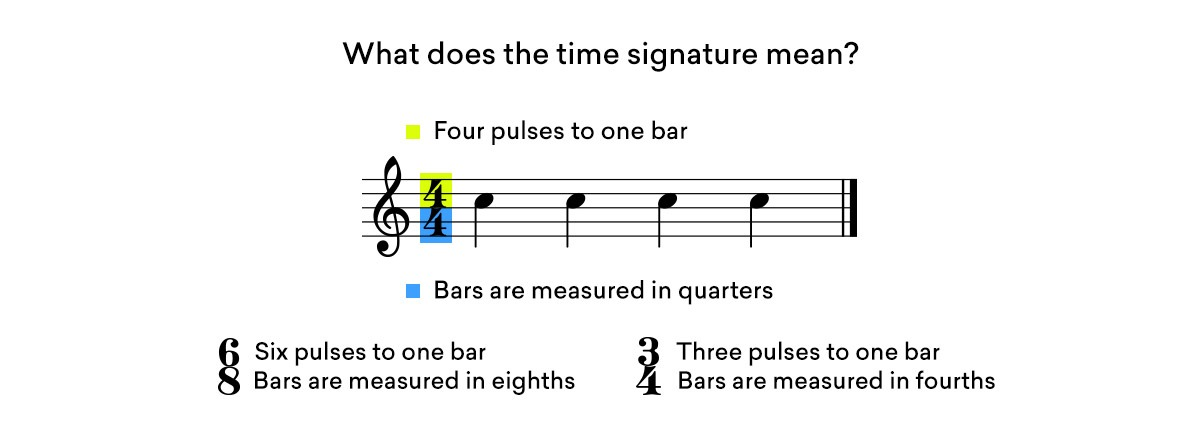
\includegraphics[width=0.8\textwidth]{images/Rythm_body}
\end{figure}

Natürlich gibt es noch viel mehr Taktarten als den 4/4-Takt. Alle Walzer sind im ¾-Takt und dann gibt es auch noch die Geschichte mit zusammengesetzten und ungeraden Taktarten.

\subsubsection{Starke und schwache Zählzeiten}
Ok, jetzt da du weißt, wie Taktarten funktionieren und Taktschläge in einen Takt passen, sollten wir uns anschauen, wie Rhythmus innerhalb eines Taktes funktioniert. Innerhalb eines Taktes gibt es starke Taktschläge, die den Puls vorantreibenund schwache Taktschläge,die dem Puls entgegenwirken. Im 4/4-Takt zum Beispiel fallen die starken Taktschläge auf die erste und dritte Viertelnote im Takt, und die schwachen Taktschläge fallen auf die zweite und vierte Viertelnote.

\begin{figure}[H]
    \centering
    
\includegraphics[width=0.8\textwidth]{images/Rythm_body_2}
\end{figure}

Im ¾-Takt fällt der starke Taktschlag auf die erste Viertelnote und die schwachen Taktschläge fallen auf die zweite und dritte Viertelnote.

\begin{figure}[H]
    \centering
    
\includegraphics[width=0.8\textwidth]{images/Rythm_body_3}
\end{figure}

Wenn du dich erstmal mit starken und schwachen Taktschlägen beschäftigt hast, hörst du sie überall. Beispiele dafür sind der EINS-zwei, EINS-zwei Puls einer Kick-Drum in einem 4/4-Disco-Song oder das EINS-zwei-drei, EINS-zwei-drei eines Walzers.

\subsubsection{Zweier- und Dreiertakte}
Bisher haben wir uns nur mit dem ¾- und 4/4-Takt, den beiden gängigsten Taktarten, beschäftigt. Falls du zusammengesetzte und ungerade Taktarten in deinem Track verwenden willst, musst du verstehen, dass Taktschläge innerhalb eines Taktes in Zweier- und Dreierpaaren gefühlt werden. Das Ganze macht mehr Sinn, wenn du weißt, wie starke und schwache Taktschläge funktionieren. Eine Art, Dreier- und Zweiertakte zu visualisieren, besteht darin, sich den Unterschied zwischen einem rollenden Dreieck und einem rollenden Quadrat vorzustellen, bei dem mit jeder neuen Umdrehung ein starker Taktschlag fällt.

Wenn du dir die starken und schwachen Taktschläge in einem 4/4-Takt anschaust, kannst du sie in zwei Zweier-gruppen unterteilen – stark – schwach, stark – schwach.

\begin{figure}[H]
    \centering
    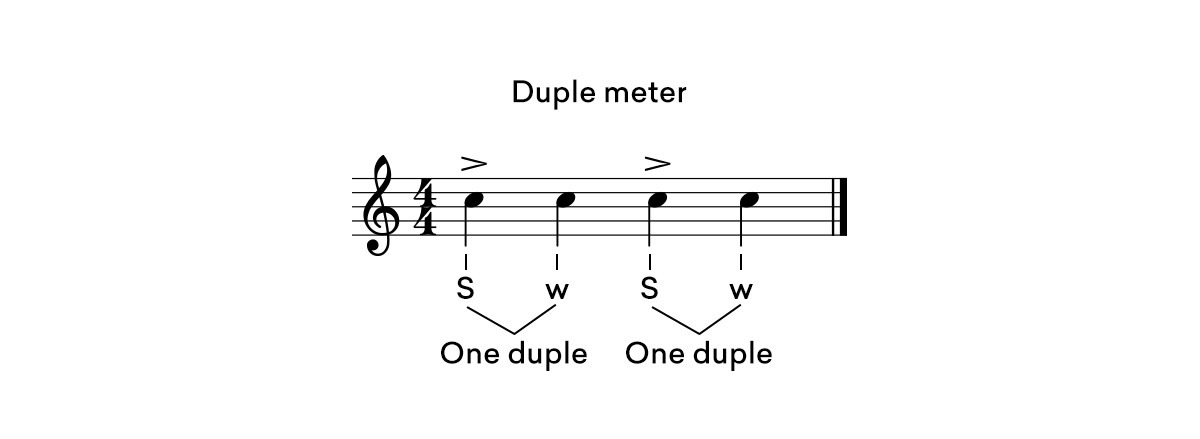
\includegraphics[width=0.8\textwidth]{images/Rythm_body_4}
\end{figure}

Ein stark-schwach-Muster bedeutet, dass es sich um einen Zweiertakt handelt. Da er in zwei Zweierpaare unterteilt ist, wird der 4/4-Takt manchmal auch Quadrupel-Takt genannt. Im ¾-Takt gibt es nur eine Dreiergruppe – stark – schwach – schwach.

\begin{figure}[H]
    \centering
    
\includegraphics[width=0.8\textwidth]{images/Rythm_body_5}
\end{figure}

Ein stark-schwach-schwach-Muster bedeutet, dass es sich um einen Dreiertakt handelt. Jedes rhythmische Muster und jeder Takt kann in Zweier- oder Dreiermetren unterteilt werden.

\subsubsection{Simple vs. zusammengesetzte Taktarten}
Simple und zusammengesetzte Taktarten hängen direkt mit dem Metrum zusammen. Das Metrum legt fest, wie der Rhythmus anhand von starken und schwachen Taktschlägen gefühlt wird. Simple und zusammengesetzte Taktarten bestimmen, ob eine Einheit aus kürzeren Noten (meistens Achtelnoten) in Zweier- oder Dreiergruppen aufgeteilt wird. Simple Taktarten gruppieren Achtelnoten in Zweiergruppen. Der 4/4-Takt ist ein simpler Zweiertakt. Seine Achtelnoten werden gezählt als EINS-und, zwei-und, DREI-und, vier-und.

\begin{figure}[H]
    \centering
    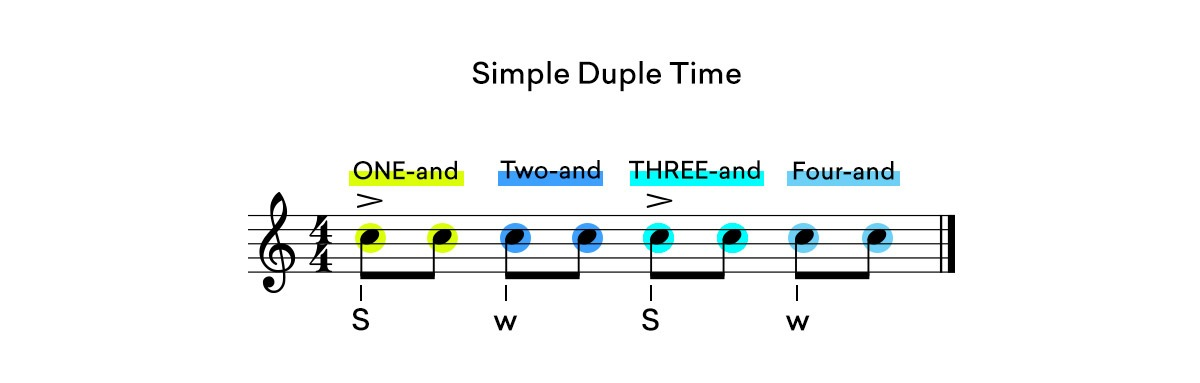
\includegraphics[width=0.8\textwidth]{images/Rythm_body_6}
\end{figure}

Der ¾-Takt ist ein simpler Dreiertakt. Er wird gezählt als EINS-und, zwei-und, drei-und.

\begin{figure}[H]
    \centering
    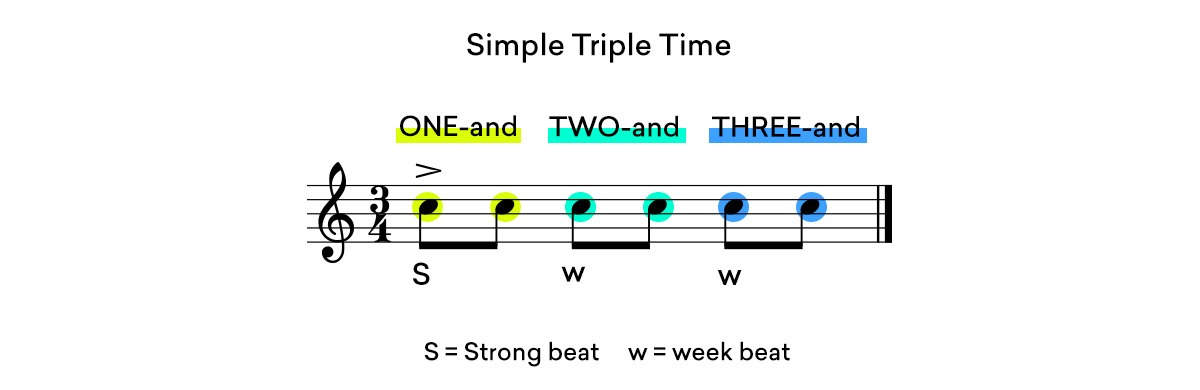
\includegraphics[width=0.8\textwidth]{images/Rythm_body_7}
\end{figure}

Zusammengesetzte Taktarten gruppieren Achtelnoten in Dreiergruppen. 6/8 und 9/8 sind beide Beispiele für eine zusammengesetzte Taktart. Im zusammengesetzten 6/8-Zweiertakt werden die Noten in zwei Gruppen aus jeweils drei Achtelnoten unterteilt.

\begin{figure}[H]
    \centering
    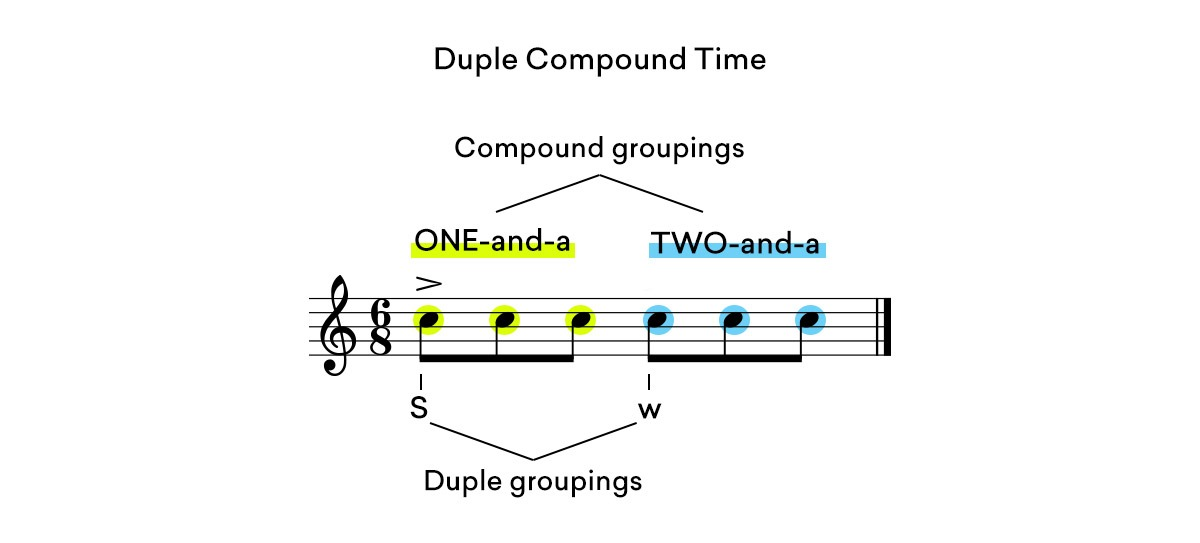
\includegraphics[width=0.8\textwidth]{images/Rythm_body_8}
\end{figure}

Die Achtelnoten könnten somit als EINS-und-a, ZWEI-und-a gezählt werden. Drakes Song Plastic Bag ist ein tolles Beispiel für einen Pop-Song, der dem 6/8-Rhythmus folgt. Im zusammengesetzten 9/8-Dreiertakt sind die Noten in drei Gruppen aus drei Achtelnoten unterteilt.

\begin{figure}[H]
    \centering
    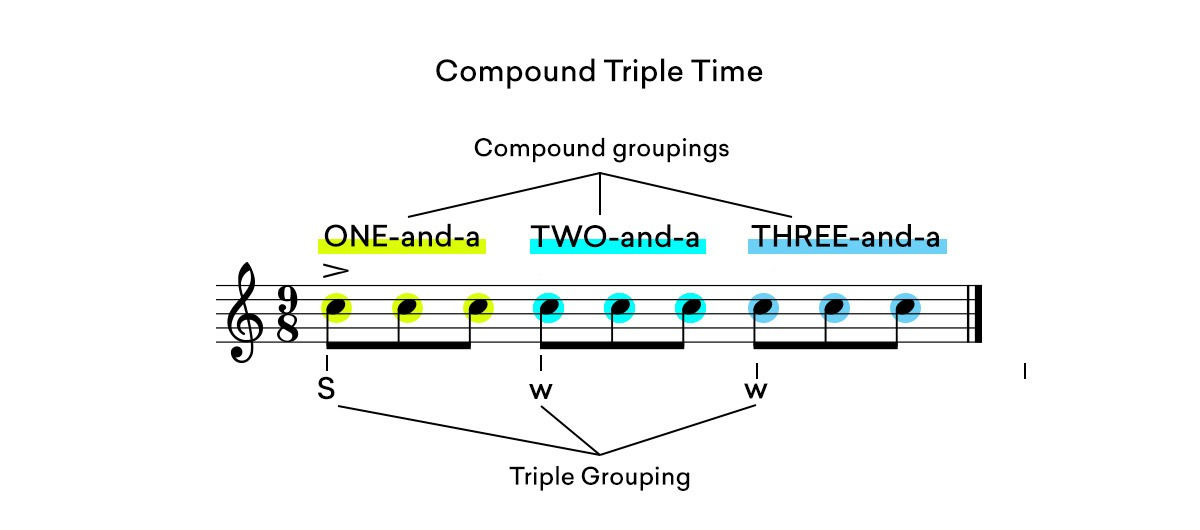
\includegraphics[width=0.8\textwidth]{images/Rythm_body_9}
\end{figure}

Die Achtelnoten werden gezählt als EINS-und-a, ZWEI-und-a, DREI-und-a. Der berühmte Jazz-Track Blue Rondo A La Turk von Dave Brubeck ist ein gutes Beispiel für den 9/8-Takt. Der Rhythmus in diesem Track wechselt zwischen dem zusammengesetzten und ungeraden 9/8-Takt. Finde heraus, ob den den Unterschied hören kannst!

\subsubsection{Ungerade Taktarten}
Ungerade Takte können etwas einschüchternd sein, es gibt viel zu wissen auf diesem Gebiet. Doch wenn du erstmal weißt, wie Zweier- und Dreiermetren funktionieren, kommst du auch mit jedem ungeraden Takt klar. Ungerade Taktarten gehen noch viel weiter mit den Regeln als simple und zusammengesetzte Taktarten, indem sie sie kombinieren. Das liegt daran, dass alle ungeraden Taktarten einem Muster folgen, das auf einer Kombination aus Zweier- und Dreiergruppen basiert. Schauen wir uns den 5{/8}-Takt an. Er kann entweder aus einer Zweiergruppe plus einer Dreiergruppe bestehen, oder einer Dreiergruppe plus einer Zweiergruppe.

\begin{figure}[H]
    \centering
    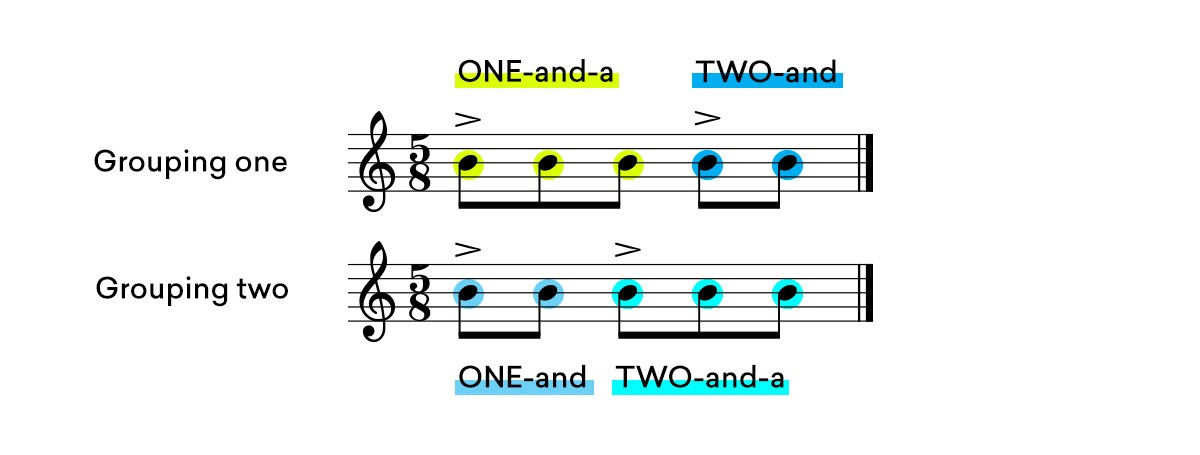
\includegraphics[width=0.8\textwidth]{images/Rythm_body_10}
\end{figure}

Falls das deiner Meinung nach keinen Sinn ergibt, versuche es einfach damit, das Metrum laut mitzuzählen, jedoch nur in Dreier- und Zweiergruppen. Für einen  5/8-Takt würdest du dementsprechend entweder EINS-und ZWEI-und-a zählen, oder EINS-und-a ZWEI-und. Wenn wir uns wieder Blue Rondo A La Turk als Beispiel ansehen, dann folgt der 9/8-Teil als ungerader Takt dem Muster EINS-und, ZWEI-und, DREI-und, VIER-und-a.

\begin{figure}[H]
    \centering
    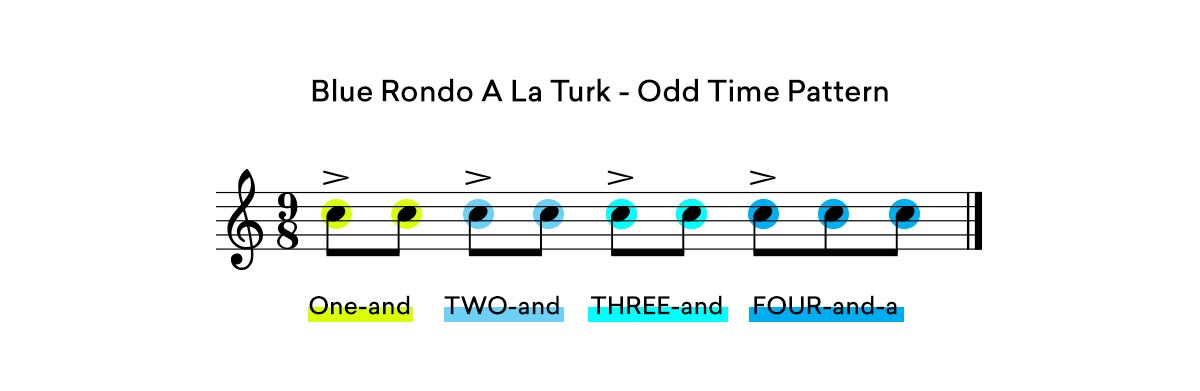
\includegraphics[width=0.8\textwidth]{images/Rythm_body_11}
\end{figure}

\end{document}